\documentclass[11pt]{article}

\usepackage{graphicx}
\usepackage{wrapfig}
\usepackage{url}
\usepackage{wrapfig}
\usepackage{hyperref} 
\usepackage{color}
\usepackage{amsfonts}
\usepackage{amssymb}
\usepackage{amstext}
\usepackage{enumerate}
\usepackage{amsmath,bm}
\oddsidemargin 0mm
\evensidemargin 5mm
\topmargin -20mm
\textheight 240mm
\textwidth 160mm




\newcommand{\vw}{{\bf w}}
\newcommand{\vx}{{\bf x}}
\newcommand{\vy}{{\bf y}}
\newcommand{\vxi}{{\bf x}_i}
\newcommand{\yi}{y_i}
\newcommand{\vxj}{{\bf x}_j}
\newcommand{\vxn}{{\bf x}_n}
\newcommand{\yj}{y_j}
\newcommand{\ai}{\alpha_i}
\newcommand{\aj}{\alpha_j}
\newcommand{\X}{{\bf X}}
\newcommand{\Y}{{\bf Y}}
\newcommand{\vz}{{\bf z}}
\newcommand{\msigma}{{\bf \Sigma}}
\newcommand{\vmu}{{\bf \mu}}
\newcommand{\vmuk}{{\bf \mu}_k}
\newcommand{\msigmak}{{\bf \Sigma}_k}
\newcommand{\vmuj}{{\bf \mu}_j}
\newcommand{\msigmaj}{{\bf \Sigma}_j}
\newcommand{\pij}{\pi_j}
\newcommand{\pik}{\pi_k}
\newcommand{\D}{\mathcal{D}}
\newcommand{\el}{\mathcal{L}}
\newcommand{\N}{\mathcal{N}}
\newcommand{\vxij}{{\bf x}_{ij}}
\newcommand{\vt}{{\bf t}}
\newcommand{\yh}{\hat{y}}
\newcommand{\code}[1]{{\footnotesize \tt #1}}
\newcommand{\alphai}{\alpha_i}
\graphicspath{ {pic/} }


\pagestyle{myheadings} 
%\markboth{Homework 2}{Fall 2015 CS 475 Machine Learning: Homework 2} 


\title{CS 435 Artificial Intelligence: Homework 2\\Game Playing\\}
\author{Li-Yi Lin / llin34@jhu.edu}

\begin{document}
\maketitle
%%%%%%%%%%%%%%%%%%%%%%%%%%%%%%%%%%%%%%%%%%%%%%%%%%%%%%%%%%%
\noindent
\textbf{Question 1-Depth First Search (DFS)}\\
The Depth First Search (DFS) will keep searching the path to the destination by first exploring the neighbor nodes that have not been reached. It doesn't care about the cost. Therefore, DFS will not necessarily find the optimal solution. \\

\noindent
\textbf{tinyMaze: }\\
$[$SearchAgent$]$ using function depthFirstSearch\\
$[$SearchAgent$]$ using problem type PositionSearchProblem\\
Path found with total cost of 10 in 0.0 seconds\\
Search nodes expanded: 14\\
Pacman emerges victorious! Score: 500\\
Average Score: 500.0\\
Scores:        500.0\\
Win Rate:      1/1 (1.00)\\
Record:        Win\\

\noindent
\textbf{mediumMaze:}\\
$[$SearchAgent$]$: using function depthFirstSearch\\
$[$SearchAgent$]$: using problem type PositionSearchProblem\\
Path found with total cost of 130 in 0.0 seconds\\
Search nodes expanded: 144\\
Pacman emerges victorious! Score: 380\\
Average Score: 380.0\\
Scores:        380.0\\
Win Rate:      1/1 (1.00)\\
Record:        Win\\

\noindent
\textbf{bigMaze:}\\
$[$SearchAgent$]$: using function depthFirstSearch\\
$[$SearchAgent$]$ using problem type PositionSearchProblem\\
Path found with total cost of 210 in 0.0 seconds\\
Search nodes expanded: 390\\
Pacman emerges victorious! Score: 300\\
Average Score: 300.0\\
Scores:        300.0\\
Win Rate:      1/1 (1.00)\\
Record:        Win\\

%%%%%%%%%%%%%%%%%%%%%%%%%%%%%%%%%%%%%%%%%%%%%%%%%%%%%%%%%%%
\newpage
\noindent
\textbf{Question 2-Breadth First Search (BFS)}\\
If the cost of every step is the same, then BFS will always find the optimal path (with lowest cost) from the starting position to the destination.\\

\noindent
\textbf{tinyMaze:}\\
$[$SearchAgent$]$ using function bfs\\
$[$SearchAgent$]$ using problem type PositionSearchProblem\\
Path found with total cost of 8 in 0.0 seconds\\
Search nodes expanded: 15\\
Pacman emerges victorious! Score: 502\\
Average Score: 502.0\\
Scores:        502.0\\
Win Rate:      1/1 (1.00)\\
Record:        Win\\

\noindent
\textbf{mediumMaze:}\\
$[$SearchAgent$]$ using function bfs\\
$[$SearchAgent$]$ using problem type PositionSearchProblem\\
Path found with total cost of 68 in 0.0 seconds\\
Search nodes expanded: 269\\
Pacman emerges victorious! Score: 442\\
Average Score: 442.0\\
Scores:        442.0\\
Win Rate:      1/1 (1.00)\\
Record:        Win\\

\noindent
\textbf{bigMaze:}\\
$[$SearchAgent$]$ using function bfs\\
$[$SearchAgent$]$ using problem type PositionSearchProblem\\
Path found with total cost of 210 in 0.1 seconds\\
Search nodes expanded: 620\\
Pacman emerges victorious! Score: 300\\
Average Score: 300.0\\
Scores:        300.0\\
Win Rate:      1/1 (1.00)\\
Record:        Win\\

%%%%%%%%%%%%%%%%%%%%%%%%%%%%%%%%%%%%%%%%%%%%%%%%%%%%%%%%%%%
\newpage
\noindent
\textbf{Grad Stucent-Iterative Eeepening Search:}\\
\textbf{tinyMaze:}\\
$[$SearchAgent$]$ using function ids\\
$[$SearchAgent$]$ using problem type PositionSearchProblem\\
Path found with total cost of 10 in 0.0 seconds\\
Search nodes expanded: 86\\
Pacman emerges victorious! Score: 500\\
Average Score: 500.0\\
Scores:        500.0\\
Win Rate:      1/1 (1.00)\\
Record:        Win\\

\noindent
\textbf{mediumMaze:}\\
$[$SearchAgent$]$ using function ids\\
$[$SearchAgent$]$ using problem type PositionSearchProblem\\
Path found with total cost of 68 in 0.2 seconds\\
Search nodes expanded: 8138\\
Pacman emerges victorious! Score: 442\\
Average Score: 442.0\\
Scores:        442.0\\
Win Rate:      1/1 (1.00)\\
Record:        Win\\

\noindent
\textbf{bigMaze:}\\
$[$SearchAgent$]$ using function ids\\
$[$SearchAgent$]$ using problem type PositionSearchProblem\\
Path found with total cost of 210 in 1.4 seconds\\
Search nodes expanded: 60211\\
Pacman emerges victorious! Score: 300\\
Average Score: 300.0\\
Scores:        300.0\\
Win Rate:      1/1 (1.00)\\
Record:        Win\\

%%%%%%%%%%%%%%%%%%%%%%%%%%%%%%%%%%%%%%%%%%%%%%%%%%%%%%%%%%%
\newpage
\noindent
\textbf{Question 3-Uniform Cost Search (UCS):}\\
\textbf{mediumMaze:}\\
$[$SearchAgent$]$ using function ucs\\
$[$SearchAgent$]$ using problem type PositionSearchProblem\\
Path found with total cost of 68 in 0.1 seconds\\
Search nodes expanded: 269\\
Pacman emerges victorious! Score: 442\\
Average Score: 442.0\\
Scores:        442.0\\
Win Rate:      1/1 (1.00)\\
Record:        Win\\

\noindent
\textbf{mediumDottedMaze:}\\
Path found with total cost of 1 in 0.0 seconds\\
Search nodes expanded: 186\\
Pacman emerges victorious! Score: 646\\
Average Score: 646.0\\
Scores:        646.0\\
Win Rate:      1/1 (1.00)\\
Record:        Win\\

\noindent
\textbf{mediumScaryMaze:}\\
Path found with total cost of 68719479864 in 0.0 seconds\\
Search nodes expanded: 108\\
Pacman emerges victorious! Score: 418\\
Average Score: 418.0\\
Scores:        418.0\\
Win Rate:      1/1 (1.00)\\
Record:        Win\\

%%%%%%%%%%%%%%%%%%%%%%%%%%%%%%%%%%%%%%%%%%%%%%%%%%%%%%%%%%%
\newpage
\noindent
\textbf{Grad Stucent-New Cost Fuction for UCS:}\\
In this question set, I implemented a new cost function for UCS algorithm to solve the maze problem. The new cost function considers two modes of cost calculation: one is for finding all the food, and another is for escapeing the nearby ghosts. The cost function will fist find the nearest food and ghost and compare the distances from the current position to them. If the distance between the nearest ghost and the current position is short than that of the nearest food, then the mode will be "escape". Otherwise, the mode will be "eat". The mode will switch during the searching process according to the position of the pacman.\\

\noindent
In the "eat" mode, the cost will simply be the manhattan distance between the nearest food and the current position of the pacman. In the "escape" mode, the cost function will first find the nearest ghosts locat at each side (north, south, east, and west) of the pacman. If the nearest ghost is at the north side, then the cost function will assign more cost when the next state is going north (one ghost might belong to two sides of the pacman). For finding the nearest ghost at the north side, the equation will be 
$$\text{northNearest = maxX + maxY - util.manhattanDistance(pos, g)}$$
where "pos" is the current position of the pacman, "g" is the position of a ghost, and maxX and maxY are the length and width of the maze. The more the value, the nearer the ghost is. The cost function will use the same equation to find the value of each ghost at four sides. The cost function will then assign cost according to vertical direction and horizontal direction. And when the nearest ghost is at the north or south side, the cost for ghost will be:
$$\text{ghostCost += (northNearest + 1.0) / (southNearest + 1.0)}$$
Or, if the nearest ghost is at the east or west side, the cost for the ghost will be:
$$\text{ghostCost += (eastNearest + 1.0) / (westNearest + 1.0)}$$
The intuition for these equation is from the "StayEastSearchAgent" and "StayWestSearchAgent". For example, when a nearest ghost is at the north side, then "northNearest" must be larger than "southNearest". So when next step is going north, the cost will increase. Hence, it will encourage the pacman to go south.\\

\noindent
If the cost function only considers the food, then the pacman will encounter the ghost very easily. So the problem is divided into several subproblems. Some part of the searching process is escaping the ghost, and when the ghost is far away, the searching process will switch to finding foods. Although this cost function might make the pacman to walk more steps, it can make the pacman safer since the pacman can have the ghost-escaping ability. This assigment only calculate the cost and find the path before the game starts. If it can recalculate the cost each time when the ghosts move, that might be more interesting.\\

\noindent
\textbf{mediumMaze:}\\
Path found with total cost of 68 in 0.0 seconds\\
Search nodes expanded: 259\\
Pacman emerges victorious! Score: 442\\
Average Score: 442.0\\
Scores:        442.0\\
Win Rate:      1/1 (1.00)\\
Record:        Win\\

\noindent
\textbf{mediumDottedMaze:}\\
Path found with total cost of 74 in 0.0 seconds\\
Search nodes expanded: 146\\
Pacman emerges victorious! Score: 646\\
Average Score: 646.0\\
Scores:        646.0\\
Win Rate:      1/1 (1.00)\\
Record:        Win\\

\noindent
\textbf{mediumScaryMaze:}\\
Path found with total cost of 92 in 0.0 seconds\\
Search nodes expanded: 222\\
Pacman emerges victorious! Score: 418\\
Average Score: 418.0\\
Scores:        418.0\\
Win Rate:      1/1 (1.00)\\
Record:        Win\\


%%%%%%%%%%%%%%%%%%%%%%%%%%%%%%%%%%%%%%%%%%%%%%%%%%%%%%%%%%%
\newpage
\noindent
\textbf{Question 4-A* search using manhattanHeuristic:}\\
\textbf{tinyMaze:}\\
$[$SearchAgent$]$ using function astar and heuristic manhattanHeuristic\\
$[$SearchAgent$]$ using problem type PositionSearchProblem\\
Path found with total cost of 8 in 0.0 seconds\\
Search nodes expanded: 14\\
Pacman emerges victorious! Score: 502\\
Average Score: 502.0\\
Scores:        502.0\\
Win Rate:      1/1 (1.00)\\
Record:        Win\\

\noindent
\textbf{mediumMaze:}\\
$[$SearchAgent$]$ using function astar and heuristic manhattanHeuristic\\
$[$SearchAgent$]$ using problem type PositionSearchProblem\\
Path found with total cost of 68 in 0.0 seconds\\
Search nodes expanded: 222\\
Pacman emerges victorious! Score: 442\\
Average Score: 442.0\\
Scores:        442.0\\
Win Rate:      1/1 (1.00)\\
Record:        Win\\

\noindent
\textbf{bigMaze:}\\
$[$SearchAgent$]$ using function astar and heuristic manhattanHeuristic\\
$[$SearchAgent$]$ using problem type PositionSearchProblem\\
Path found with total cost of 210 in 0.2 seconds\\
Search nodes expanded: 549\\
Pacman emerges victorious! Score: 300\\
Average Score: 300.0\\
Scores:        300.0\\
Win Rate:      1/1 (1.00)\\
Record:        Win\\

%%%%%%%%%%%%%%%%%%%%%%%%%%%%%%%%%%%%%%%%%%%%%%%%%%%%%%%%%%%
\newpage
\noindent
\textbf{Question 5-Solves the corners problem with a BFS agent:}\\
\textbf{tinyCorners:}\\
$[$SearchAgent$]$ using function bfs\\
$[$SearchAgent$]$ using problem type CornersProblem\\
Path found with total cost of 28 in 0.0 seconds\\
Search nodes expanded: 252\\
Pacman emerges victorious! Score: 512\\
Average Score: 512.0\\
Scores:        512.0\\
Win Rate:      1/1 (1.00)\\
Record:        Win\\

\noindent
\textbf{mediumCorners:}\\
$[$SearchAgent$]$ using function bfs\\
$[$SearchAgent$]$ using problem type CornersProblem\\
Path found with total cost of 106 in 0.2 seconds\\
Search nodes expanded: 1966\\
Pacman emerges victorious! Score: 434\\
Average Score: 434.0\\
Scores:        434.0\\
Win Rate:      1/1 (1.00)\\
Record:        Win\\

%%%%%%%%%%%%%%%%%%%%%%%%%%%%%%%%%%%%%%%%%%%%%%%%%%%%%%%%%%%
\newpage
\noindent
\textbf{Grad Student-Heuristic for corner problem}\\
For the corner problem, I implemented a new heuristic that needs 169 and 701 search nodes expanded for "tinyCorners" and "mediumCorners" respectively (for more detail, please see the result shown below). The basic idea of the heuristic is that it will keep accumulating the manhattan distance between the current position to the nearest unvisited corner and from the nearest unvisited corner to its nearest unvisited corner and so on until all the corners have been reached. See the following example:\\

\begin{center}
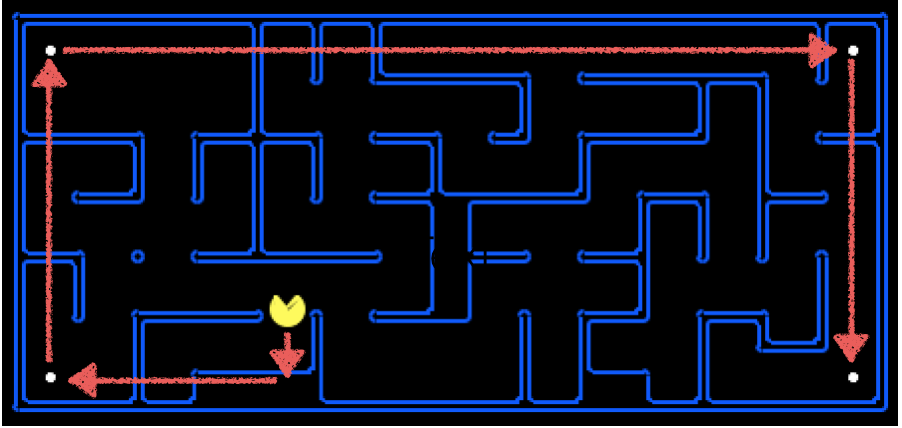
\includegraphics[scale=0.8]{cornerHeuristic}\\
\end{center}

\noindent
The red line means the manhattan distance and the arrow means the order that it finds the corners. I designed this heuristic because I thought that the cost should not only relate to the nearest unvisited corner but also relate to other unvisited corners. This algorithm is a consistent cost function since when the pacman walks one step, the cost will change at most one and the cost for one step is one, making $h(n) \leq c(n, a, n') + h(n')$ hold true.\\

\noindent
\textbf{tinyCorners:}\\
Path found with total cost of 30 in 0.0 seconds\\
Search nodes expanded: 201\\
Pacman emerges victorious! Score: 510\\
Average Score: 510.0\\
Scores:        510.0\\
Win Rate:      1/1 (1.00)\\
Record:        Win\\

\noindent
\textbf{mediumCorners:}\\
Path found with total cost of 106 in 0.2 seconds\\
Search nodes expanded: 736\\
Pacman emerges victorious! Score: 434\\
Average Score: 434.0\\
Scores:        434.0\\
Win Rate:      1/1 (1.00)\\
Record:        Win\\


%%%%%%%%%%%%%%%%%%%%%%%%%%%%%%%%%%%%%%%%%%%%%%%%%%%%%%%%%%%
\newpage
\noindent
\textbf{Question 7-Solves the eating all the dots problem with A* with a null heuristic:}\\
\textbf{testSearch:}\\
$[$SearchAgent$]$ using function astar and heuristic nullHeuristic\\
$[$SearchAgent$]$ using problem type FoodSearchProblem\\
Path found with total cost of 7 in 0.0 seconds\\
Search nodes expanded: 14\\
Pacman emerges victorious! Score: 513\\
Average Score: 513.0\\
Scores:        513.0\\
Win Rate:      1/1 (1.00)\\
Record:        Win\\

\noindent
\textbf{trickySearch}\\
$[$SearchAgent$]$ using function astar and heuristic nullHeuristic\\
$[$SearchAgent$]$ using problem type FoodSearchProblem\\
Path found with total cost of 60 in 75.8 seconds\\
Search nodes expanded: 16688\\
Pacman emerges victorious! Score: 570\\
Average Score: 570.0\\
Scores:        570.0\\
Win Rate:      1/1 (1.00)\\
Record:        Win\\

%%%%%%%%%%%%%%%%%%%%%%%%%%%%%%%%%%%%%%%%%%%%%%%%%%%%%%%%%%%
\newpage
\noindent
\textbf{Grad Student-Solves the eating all the dots problem with A* with a foodHeuristic:}\\
Description\\



\noindent
\textbf{testSearch:}\\
Path found with total cost of 7 in 0.0 seconds\\
Search nodes expanded: 12\\
Pacman emerges victorious! Score: 513\\
Average Score: 513.0\\
Scores:        513.0\\
Win Rate:      1/1 (1.00)\\
Record:        Win\\

\noindent
\textbf{trickySearch:}\\
Path found with total cost of 60 in 17.0 seconds\\
Search nodes expanded: 7209\\
Pacman emerges victorious! Score: 570\\
Average Score: 570.0\\
Scores:        570.0\\
Win Rate:      1/1 (1.00)\\
Record:        Win\\



\end{document}

